% ----------------------------------------------------------------------------
% Copyright (c) 2016 by Burkhardt Renz. All rights reserved.
% Die Vorlage für eine Abschlussarbeit in der Informatik am Fachbereich
% MNI der THM ist lizenziert unter einer Creative Commons
% Namensnennung-Nicht kommerziell 4.0 International Lizenz.
%
% Id:$
% ----------------------------------------------------------------------------

\chapter{Design}
\label{chapter:Design}
In diesem Kapitel werden die in \cref{chapter:Problembeschreibung} beschriebenen Problemstellung bearbeitet. Anfänglich werden Designziele definiert, die den Rahmen für die Konzipierung bilden. In \cref{section:Datenmodell} wird ein Datenmodell vorgestellt, welches sich an Standards von bereits existierenden Tracingmodellen orientiert. \cref{section:Verarbeitungsmodell} präsentiert ein Konzept zur verarbeitung der erhobenen Tracingdaten. Der \cref{section:Visualisierung} beschäftigt sich mit der Darstellung der Tracingdaten zur Informationsgewinnen durch den Anwender der Bibliothek. Somit wird ein Konzept für die Tracinginfrastruktur \textbf{Traktor }zur Erhebung, Verarbeitung und Visualisierung von Tracingdaten vorgestellt.

\section{Designziele}
\label{section:Designziele}

Aus den in \cref{section:Anforderungsanalyse} beschriebenen Anforderungen folgern Designziele, die an das Design gestellt werden. Die von Google erstellte Fachpublikation \emph{Dapper, a Large-Scale Distributed Systems Tracing Infrastrcture} dient vielen Tracingsystemen als konzeptionelle Grundlage. In der Puplikation werden Designziele aufgeführt, die neue Tracingsysteme bewerten sollten. Es werden Designziele bewertet, die von Dapper genannt werden. Ausserdem sind zusätzliche Designziele aufgezeigt, die aus den Anforderungen des verteilten rendering Systems hervorkommen. Diese Designziele umfassen die (\lowroman{1}) \textbf{Verarbeitungskosten}, die (\lowroman{2}) \textbf{Benutzbarkeit}, die (\lowroman{3}) \textbf{Portabilität} und die (\lowroman{4}) \textbf{Datenverfügbarkeit}. Ausserdem werden Nicht-Ziele definiert. Zu diesen gehören die (\lowroman{5}) \textbf{Anwendungs-Level Transparenz} und die (\lowroman{6}) \textbf{Skalierbarkeit}.

\subsection{Ziele}
\label{subsection:Ziele}
\textbf{Verarbeitungskosten} \space\space\space Ein für die Performance der Anwendung kritisches Designziel, in der Tracing eingeführt werden soll, stellt der \textbf{Overhead} dar. Der Overhead, der durch die Instrumentalisierung entsteht, soll möglichst gering sein. So kann etwa in spezialisierten hochperfomanten Services kleinster, durch Instrumentalisierung entstehender Mehraufwand, deutlich merkbar sein.\footpartcite{Shanbhag2010}. 

\textbf{Benutzbarkeit} \space\space\space Die Benutzbarkeit des Tracingsystems soll durch die Verwendung von Standards gewährleistet sein. Die von \emph{Opentracing} veröffentlichte \gls{apiLabel} soll der Instrumentalisierungsbibliothek eine vertraute und bewährte Anwendererfahrung liefern. 

\textbf{Portabilität} \space\space\space Ein weiteres Designziel soll eine gegebene \textbf{Portabilität} sein. Die Umgebung für die das Tracingsystem entwickelt wird, ist eine Mischung aus Platformabhängigen und Platformunabhängigen Komponenten. Durch den verminderten Mehraufwand der bei platformunabhängigen Komponeten entsteht, wird eine verbesserte Nutzerfreundlichkeit gewährleistet. Vorallem bei der Integration in bestehende Systeme wird dies bemerkbar, da Bauprozesse von Projekten platformabhängig sind. Der platformabhängige Bauprozess soll im Falle des verteilten rendering System nicht beeinflusst werden. Die 

\textbf{Datenverfügbarkeit} \space\space\space Die Datenverfügbarkeit soll zeitnah stattfinden. Die von der Tracinginfrastruktur generierten Tracingdaten sollen zur Laufzeit darsgestellt werden. 

\subsection{Nicht-Ziele}
\label{subsection:Nicht-Ziele}

Die von Dapper genannten Designziele der \emph{Anwendungs-Level Transparenz} und der \emph{Skalierbarkeit} spielen für das verteilte rendering System eine untergeordnete Rolle. Diese Bewertung hat ihren Ursprung aus einer interpretierten Form eines Sprichworts. 

\begin{quote}
	Du bist nicht Google, also versuch auch nicht Google zu sein
\end{quote}

Dapper ist für eine Infrastruktur konzipiert, die globalen  Maßstäben entspricht. Das verteilte rendering System entspricht nicht diesen Maßstäben, somit soll auch die Tracinginfrastruktur diese nicht erfüllen müssen. Die beiden Deisgnziele von Dapper werden als Nicht-Ziele für das verteilte rendering System bewertet.

\textbf{Anwendungs-Level Transparenz}\space\space\space Instrumentalisierung erfordert eingreifen in Anwendungsquellcode. Dapper löst dies durch Ausnutzung von Bibliotheken. Diese werden Instrumentalisiert und in der Anwendungslogik verwendet. Somit ist die Tracinginfrastruktur für den Anwendungsentwickler nicht wahrnehmbar. Die Instrumentalisierung des verteilten rendering Systems soll an semantisch relevanten Bereichen stattfinden und flexibel sein. Dies gelingt durch direktes modifizieren der Anwendungslogik. Der Anwendungsentwickler muss sich dementsprechend selbst um die Instrumentalisierung kümmern. 

\textbf{Skalierbarkeit} \space\space\space Der Aufbau des verteilte rendering System ist, in seiner einfachsten Form, statisch. Das bedeutet, dass eine Skalierbarkeit keine zentrale Rolle in dem Design der Tracinginfrastruktur darstellt. Die Skalierbarkeit soll allerdings bewertet werden. 

\section{Datenmodell}
\label{section:Datenmodell}

In diesem Abschnitt wird das Problem \textbf{F1} diskutiert.
Dieses Problem erfordert die Konzipierung eines Datenmodells, welches drei Aspekte berücksichtig. Der erste Aspekt wird durch die Zeitspanne des Events selbst dargestellt. Dabei muss das Event derart repräsentiert werden, sodass eine Zeitspanne als Information daraus gewonnen werden kann. Die detailierte Darstellung wird in \cref{subsection:Spans} erläutert. Der zweite Aspekt entsteht durch die Gegebenheit eines lokalen Kontexts. Dieser wird in \cref{subsection:Tracingcontext innerhalb eines Systems} beschrieben. Der dritte Aspekt ist durch die Kommuniktion von Komponenten des Systems gegeben. Dieser wird  in \cref{subsection:Tracingcontext über Systemgrenzen} dargestellt.


Das Datenmodell beruht auf dem Spanmodell, welches in der vorher beschrieben Fachpuplikation \emph{Dapper} vorgestellt, durch die Spezifikation von \emph{Opentracing} erweitert und dem Anwendungsfall des verteilten rendering Systems und des Entwicklungsprojekts angepasst wird.

Ein Überblick über das Spanmodell wird gezeigt. Ein \emph{Trace} bildet die größte Einheit des Modells ab. Traces sind Eventsammlungen, die den Weg einer Anfrage durch ein verteiltes System darstellen.Ein Trace ist die Reise der Anfrage, wohingegen einzelne Events die Etappen dieser Reise sind. Die Events werden weiterführend als Spans bezeichnet.  Ein Trace beinhaltet ein bis beliebig viele \emph{Spans}. Ein Span ist die kleinste Einheit eines Traces. Spans bilden einen Arbeitsprozess innerhalb eines Prozesses ab. Innerhalb eines \emph{Threads} ist zu jeder Zeit nur ein Span \emph{aktiv}.


\subsection{Spans}
\label{subsection:Spans}
Um Daten zu repräsentieren und zusammenzufassen, braucht es einen Datencontainer. Die Datencontainer eines Traces sind Spans. Spans beinhalten die Daten die nötig sind, um eine Reihenfolge herzustellen. Ausserdem besteht die Möglichkeit Anwendungsinformationen, wie zum Beispiel Anwendungslogs, in Spans mitzuführen.

Ein Span kapselt folgende Informationen:
\begin{itemize}
	\item Ein Operationsnamen
	\item Ein Startzeitpunkt
	\item Ein Endzeitpunkt
	\item Ein Spankontext
\end{itemize}

\begin{figure}[!ht]
	\centering
	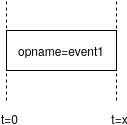
\includegraphics[scale=0.7]{img/Design/Span.png}
	\caption[Zeitliche Darstellung eines Spans]{Darstellung eines Spans mit Anfangszeit, Endzeit und Operationsnamen}
	\label{fig:Span}
\end{figure}

Der Spankontext wiederum ist auch ein Datencontainer. Dieser beinhaltet eine \emph{SpanID} und eine \emph{TraceID}. Auch ein Beziehungstyp wird mitgeführt. Der Beziehungstyp kann zum einen eine \emph{Child-of} Beziehung oder eine \emph{Follows-From} Beziehung annehmen. Die SpanID ist eine eindeutig identifizierbare Nummer, die bei der Erstellung eines Spans generiert und in dem Spankontext gespeichert wird. Die TraceID ist eine eindeutig identifizierbare Nummer, die bei der Erstellung des ersten Spans eines Traces erstellt wird. Die TraceID wird auch in dem Spankontext gespeichert. Nachfolgende Spans, die zu diesem Trace gehören, übernehmen die TraceID. Dadurch ist eine Zuordnung jedes Spans zu einem Trace gegeben. Die zeitliche Einordnung des Startzetpunktes und des Endzeitpunktes eines Spans ist in  \cref{fig:Span} dargestellt. Die Konzipierung der Start- und Endzeit sind die zentralen Daten, mit der sich Fragestellung \textbf{F1} lösen lässt. Durch die Relationbildung mittels einer Beziehungstypdefinition und der Zeitstempel, ist eine Zeitmessung von Eventzeitspannen gegeben. Das Beispiel aus \cref{fig:Eventzeitspannen} verdeutlicht dies. Die Gesamtzeit eines Events bzw. eines Spans lässt sich durch die Differenz zweier Zeitstempel ermitteln. Die Zeitspanne die von dem Span \emph{FormatiereNachricht} eingenommen wird, ergibt sich aus $t3 - t2$. Dies wäre ein Event mit einer Lebensdauer von 0.5. Die Relationstypen werden dazu genutzt, um den Zustand des Traces zu definieren. Ein Trace ist dann abgeschlossen, sobald der letzte Span eines Traces, ohne \emph{Child-Of} Beziehung beendet ist. \emph{EmpfangeAntwort} ist in diesem Fall der letzte Span. Ausserdem besitzt dieser keinen Übergeordneten Span, gegeben aus einer \emph{Follows-From} Beziehung zum Ursprungsspan. Daraus folgert der Abschluss des Traces.

\begin{figure}[!b]
	\centering
	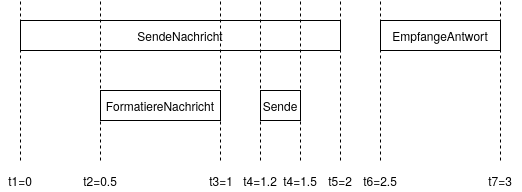
\includegraphics[scale=0.7]{img/Design/Eventzeitspannen.png}
	\caption[Zeitmessung von Spans eines Traces]{Darstellung eines Trace mit mehreren Spans. Anfangszeit und Endzeit ergeben die Gesamtzeit eines Traces}
	\label{fig:Eventzeitspannen}
\end{figure}



\subsection{Tracingcontext innerhalb eines Systems}
\label{subsection:Tracingcontext innerhalb eines Systems}

\begin{figure}[!ht]
	\centering
	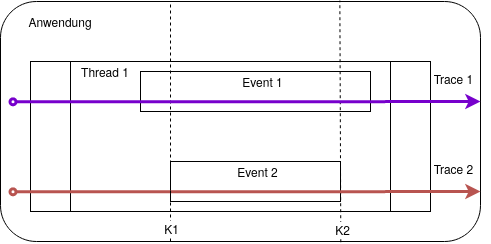
\includegraphics[scale=0.5]{img/Design/SpanThreadKontext.png}
	\caption[Tracingkontexts in einem Threads innerhalb einer Anwendung]{Anwendung mit einem Thread. Ein von der Instrumentalisierung veranlasster Kontextwechsel innerhalb eines Threads}
	\label{fig:SpanThreadKontext}
\end{figure}


Ein Prozess kann \emph{Threads} implementieren. Die Events, die in einem Thread stattfinden, können ihren Lebenszyklus entweder in diesem beginnen und beenden oder in einem Thread beginnen und in einem anderen Thread enden. Der Tracer, also die übergeordnete Verwaltungseinheit, muss jedoch jederzeit feststellen können, welches Event \emph{aktiv} ist. Der Grund dafür ist beispielsweise das Erstellen von Relationen für zu generierende Events, die ihr Elternevent kennen müssen. Eine Umgebung ist notwendig, in der der aktive Span festgestellt werden kann. Diese Umgebung wird als \emph{Scope} bezeichnet. Der Kontext eines Traces ergibt sich aus dem aktiven Span. Der Kontext ist notwendig, um folgende Spans zuordnen zu können. Anhand der aufgeführten Beispiele wird das Konzept des Scopes verdeutlicht. Dabei beinhaltet das erste Beispiel, dargestellt in \cref{fig:SpanThreadKontext}, einen Thread, indem zwei Traces parallel exisitieren. Die \cref{fig:SpanMultipleThreadKontext} stellt die Situation eines Traces über mehrere Threads dar.

Im ersten Beisiel sei gegeben, dass eine Anwendung ein Thread implementiert. Dabei exisiteren zwei parallele Traces. Trace 1 beinhaltet das Event 1. Event 1 sendet asynchron eine große Datei an ein Frontend, wie dies in dem verteilten rendering System der Fall sein könnte.  Trace 2 beinhaltet Event 2. Event 2 liest eine kleinen Datei aus einem Speicher. Es wird davon ausgegangen, dass das Schreiben deutlich mehr Zeit beansprucht, als das Lesen. Der Ablauf des Kontextwechsels beginnt mit der Erstellnug und Aktivierung des Spans, welcher Event 1 umfasst. Die Aktivierung des Spans sorgt dafür, dass dieser in dem \emph{Scope} wandert. Der Scope verwaltet den aktiven Span. Die Startzeit des Spans wird gespeichert und die Anwendungslogik asynchron bearbeitet. Event 2, welches zu Trace 2 gehört, startet und generiert den zweiten Span. Dabei findet Kontextwechsel K1 statt. K1 tauscht den Span von Event 1 mit dem Span von Event 2. Der Span von Event 2 ist nun aktiv und der Span von Event 1 nimmt implizit den Zustand \emph{nicht beendet} ein. Die Anwendungslogik, die Event 2 darstellt, wird bearbeitet. Das Event 2 beendet, woraus die Schließung des dazugehörigen Spans folgert. Die Endzeit wird gespeichert. Trace 2 schließt, da der Span von Event 2 keinen \emph{ElternID} beinhaltet und somit der Wurzelspan ist. K2 wechselt wieder den aktiven Span. Danach beendet Event 1, da der \emph{Callback}, durch die Beendigung des Schreibens, aufgerufen wird. Entsprechenden schließt Span von Event 1. Auch hier ist dieser der Elternspan und schließt Trace 1 ab. Zu jedem Zeitpunkt kann des Tracerobjekt feststelle, welches das aktive Span ist.


\begin{figure}[!ht]
	\centering
	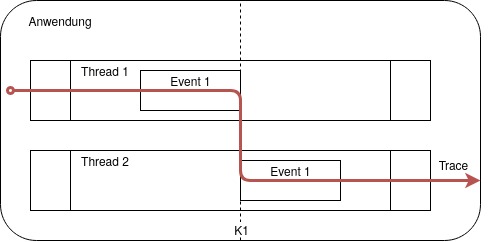
\includegraphics[scale=0.5]{img/Design/SpanMultipleThreadKontext.png}
	\caption[Tracingkontexts über mehrere Threads innerhalb einer Anwendung]{Anwendung mit zwei Threads. Ein von der Instrumentalisierung veranlasster Kontextwechsel zwischen Threads}
	\label{fig:SpanMultipleThreadKontext}
\end{figure}

Im zweiten Beispiel sei gegeben, dass eine Anwendung zwei Threads implementiert. Es exisitert ein Trace, welches Event 1 beinhaltet. Thread 1 beinhaltet Event 1. Event 1 sorgt für die die Erstellung eines Scopes in dem der Span von Event 1 erstellt und aktiviert wird. Kontextwechsel K1 findet statt. Der Scope in Thread 1 schließt. Da Event 1 in Thread 2 weitergeführt wird, beendet der Span nicht bei K1. In Thread 2 findet die Weiterführung von Event 1 statt, weshalb ein Scope eröffnet wird. In diesem Scope wird der in dem vorherigen Scope aktive Span eingeführt. Dies stellt die Kontextübermittlung dar. Event 1 endet anschließend und Trace 1 wird geschlossen.

Diese beiden Beispiele zeigen die Relevanz von Scopes zur Verfolgung des Kontexts innerhalb eines Systems ohne Netzwerkkommunikation. Scopes lösen das Problem der lokalen  Kontextverfolgbarkeit. Damit lassen sich Endzeiten von Spans innerhalb eines Systems, auch über Threadgrenzen hinaus, bestimmen. 

\subsection{Tracingcontext über Prozessgrenzen}
\label{subsection:Tracingcontext über Systemgrenzen}

Die Kontextverfolgung über Prozessgrenzen stellt wohl das schwierigste Problem im verteilten tracing dar. Im Fokus steht hierbei die Fragestellung \textbf{F3}. Es werden zwei Konzepte vorgestellt, die es ermöglichen sollen, Tracingkontext über Prozessgrenzen hinaus zu transportieren. 


\subsubsection{Registry}
Das erste Konzept ist die \textbf{Traktor Registry}. 
Der Infrastrukturaufbau, bestehend aus der Registry und der Tracer, die mit der Registry verbunden sind, erfüllt die Aufgabe der Kontextpropagierung. Die Traktor Registry dient als Nachrichtenproxy für die Tracer-Instanzen. Bei der Initialisierung einer Traktorinstanz stellt diese eine Websocketverbindung zur Registry her. Bei eingeleiteter Kontextpropagieren wird eine Websocketnachricht, die den Tracekontext beinhaltet, an die Registry gesendet. Die Registry empfängt die Nachricht und sendet diese an ihr Zieltracer weiter. Der Zieltracer, der auch eine Verbindung zur Registry aufgebaut hat, empfängt die Nachricht. Der Nachrichteninhalt wird extrahiert und für die Erstellung für kommende Spans des aktuellen Traces und der damit verbundenen Relationsbildung genutzt. Die Verarbeitungsablauf dieses Registryservices lässt sich aus \cref{fig:Traktor-Registry} erschließen.

\begin{figure}[!ht]
	\centering
	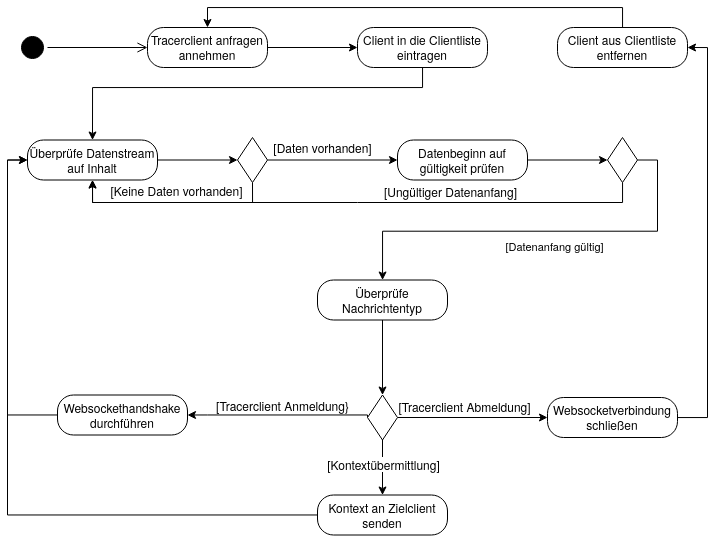
\includegraphics[scale=0.65]{img/Design/Traktor-Registry.png}
	\caption[Aktivitätendiagramm der Traktor Registry]{Aktivitätendiagramm der Traktor Registry}
	\label{fig:Traktor-Registry}
\end{figure}

\subsubsection{Interceptor}
Das zweite Konzept beruht auf dem Abfangen und dem Modifizieren von spezifizierten Nachrichten, die aus dem System gesendet werden. Es werden Betriebssystemabähngige Funktionalitäten genutzt, um ausgehende Nachrichten zu identifizieren und einzuordnen. Dabei wird auf Nachrichten gelauscht, die von einem Port ausgehen, die die Anwendungskomponente belegt. Entspricht diese Nachricht den Vorgaben, kann diese um Kontextdaten erweitert werden. Anschließend wird die Nachricht in modifizierter Form an ihren Empfänger weitergeleitet. Auf dem Empfängersystem sitzt ein gleicher \emph{Interceptor}. Dieser lauscht auf auf eingehende Nachrichten und filtert, wie beim Senden, die gewünschten Nachrichten heraus. Der Tracingkontext wird aus der Nachricht extrahiert. Anschließend wird die Nachricht, so wie sie von der Senderanwendung geschickt wurde, an die Empfängeranwendung weitergeleitet. \cref{fig:Nachrichteninterceptor} zeigt die Nachrichtenmodifikation, bei der eine Anwendung auf dem Sendersystem Nachrichten über die Ports 8080 und 8090 an eine Empfängeranwendung sendet. Ports die nicht von der Anwendung beansprucht werden, wie zum Beispiel Port 1337, sind von der Modifikation nicht betroffen. Der Interceptor erweitert die Nachrichten um den Trancingkontext, welches von dem Emfpängerinterceptor entpackt werden. Durch diese Funktionalität lässt sich die Registry, also einem potentiellen \emph{single point of failure}, ersetzten. Allerdings werden dazu auf jedem System zusätzliche, neben der Anwendung laufende, Scripte benötigt.

 \begin{figure}[!ht]
 	\centering
 	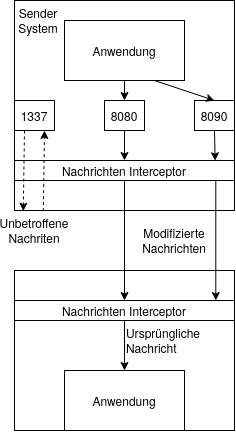
\includegraphics[scale=0.6]{img/Design/Nachrichteninterceptor.png}
 	\caption[Design des Nachrichteninterceptor]{Design des Nachrichteninterceptor}
 	\label{fig:Nachrichteninterceptor}
 \end{figure}

\section{Verarbeitungsmodell}
\label{section:Verarbeitungsmodell}
Das Verarbeitungsmodell ist das Bindeglied zwischen Visualisierung und Instrumentalisierung. Dabei sind zwei Komponenten zu designen. Die erste Komponente hat dafür zu sorgen, dass die Daten aus der Anwendung gelangen und zu einem Service übermittelt werden, der die Daten sammelt. Dafür werden \emph{Reporter} eingesetzt. Die zweite Komponente ist der \emph{Kollektor}. Dieser erhält alle Daten der Reporter. Die gesammelten Daten werden in eine strukturierte Form aufgearbeitet. Anschließend können die Daten, abhängig von der Konfiguration, gespeichert oder direkt visualisiert werden.

\subsection{Reporter}
\label{subsection:Reporter}
Bei Abschluss eines Spans wird dieser an den Reporter übermittelt. Durch eine UDP Verbindung zu dem Kollektor werden die Spans versendet. Der Trace wird von der Verwaltungseinheit parallel weitergeführt, bis dieser abgeschlossen ist. Der Reporter kennt den Zustand des gesamten Traces nicht. 

\subsection{Kollektor}
\label{subsection:Kollektor}
Der Kollektor ist ein eigener Service im verteilten System. In dem Kollektor werden die reporteten Spans gesammelt. Der Kollektor stellt einen UDP Endpunkt bereit, über den die Reporter daten übermitteln können. Diese können in einer relationalen Datenbank gespeichert werden. Das Datenmodell der Traces und Spans bietet sich dafür an. Anhand der TraceID lassen sich die dazugehörigen Spans ermitteln. Jede TraceID ist ein Eintrag in der Datenbank. Die Datenverfügbarkeit ist entsprechend gegeben.  

\section{Visualisierung}
\label{section:Visualisierung}
In diesem Kapitel sollen Darstellungsformen von Tracingdaten präsentiert werden. Dabei werden bestehende Visualisierungsmöglichkeiten von Performancedaten aufgegriffen und dem Kontext von distributed tracing, sowie dem verteilten rendering System angepasst.


\subsection{Frame Galerie}

Das verteilte Renderingsystem generiert Frames. Die Instrumentalisierung des System hat den Zweck einzelne Frames untersuchen zu können. Eine abstrakte Darstellung der Tracingdaten zur Untersuchung der Frames bietet sich daher an. Bereits existierende Tracingdarstellungen, bietet eine sehr eingeschränkte und spezifizierte Ansicht der Daten. Das Konzept der Frame Galerie soll die Daten interpretieren und für den Anwender eine Abstraktion der Tracingdaten bereitstellen. 

Das Visualisierungskonzept ist durch drei Ebenen gekennzeichnet. Jede Ebene liefert einen gewissen Grad von Informationen. Dabei bietet die oberste Ebene, dargestellt in \cref{fig:FrameGalerieObereEbene}, eine Übersicht über alle verfolgten Frames. Eine farbliche Unterscheidung hilft zusätzlich dabei, festzustellen, welche der Frames beim Clienten tatsächlich dargestellt worden sind. Nicht verwendete Frames könne beispielsweise ein Indiz für fehlerhafte Frames sein, die es weiter zu untersuchen gilt.

\begin{figure}[!ht]
	\centering
	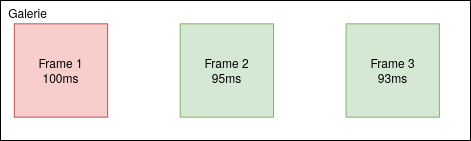
\includegraphics[scale=0.8]{img/Design/FrameGalerieObereEbene.png}
	\caption[Oberste Ebene der Frame Galerie]{ Skizzierung der oberste Ebene der Frame Galerie}
	\label{fig:FrameGalerieObereEbene}
\end{figure}

Da das verteilte rendering System Frames aus Teilframes zusammenstellt, ist es sinnvoll, den Generierungsprozess der fertigestellten Frames nachvollziehen zu können. Die mittlere Ebene, dargestellt in \cref{fig:FrameGalerieMittlereEbene},  veranschauchlicht dies durch ein Stammbaum. Wie auch bei der oberen Ebene, müssen nicht alle Teilframes, aufgrund ihres zeitlichen Auftretens in der Generierungsphase, bei der Zusammenstellung verwendet werden. Diese sind auch hier farblich gekennzeichnet. Zusätzlich sind die Generierungszeiten aus den Tracingdaten hergeleitet und an die jeweiligen Frames geheftet.

\begin{figure}[!ht]
	\centering
	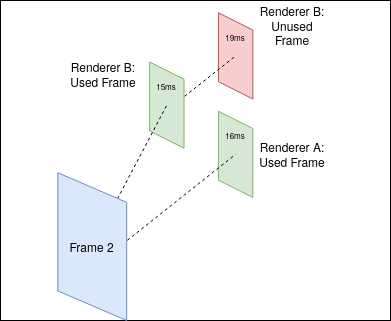
\includegraphics[scale=0.8]{img/Design/FrameGalerieMittlereEbene.png}
	\caption[Mittlere Ebene der Frame Galerie]{ Skizzierung der mittleren Ebene der Frame Galerie}
	\label{fig:FrameGalerieMittlereEbene}
\end{figure}

Die unterste Ebene ist Detailansicht der Spans. Hierzu wird die klassiche Visualisierungform von Tracingdaten verwendet. Die Servicenamen, die Operationsnamen und die dazugehörigen Verarbeitungszeiten der Spans sind erkenntlich. Zusätzlich können \emph{Breakpoints} gekennzeichnet werden. Durch Visualisierung von beispielsweise gestrichelten Linien, wie in \cref{fig:FrameGalerieUntereEbene1} gezeigt, ist ersichtlich, dass Frames, die ab diesem Zeitpunkt generiert werden, für die Zusammenführung ungenutzt bleiben.

Dem Anwender der Visualisierung ist durch die Ebenenaufteilung möglich, für ihn interessante Aspekte auszuwählen und gegebenenfalls Fehlerquellen weitergehend zu untersuchen.

\begin{figure}[!ht]
	\centering
	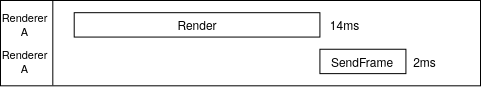
\includegraphics[scale=0.8]{img/Design/FrameGalerieUntereEbene2.png}
	\caption[Untere Ebene der Frame Galerie: Beispiel 2]{ Skizzierung der unteren Ebene von Teilframe aus Renderer A}
	\label{fig:FrameGalerieUntereEbene1}
\end{figure}
\begin{figure}[!ht]
	\centering
	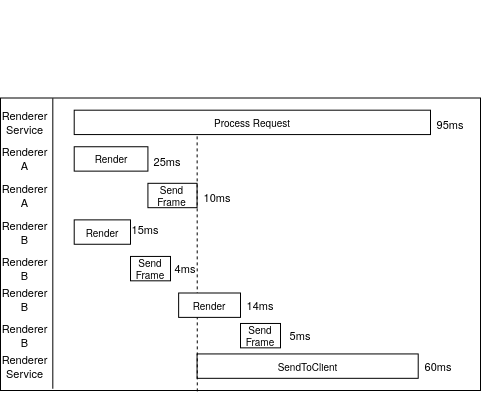
\includegraphics[scale=0.8]{img/Design/FrameGalerieUntereEbene1.png}
	\caption[Untere Ebene der Frame Galerie: Beispiel 1]{ Skizzierung der unteren Ebene von Frame 2}
	\label{fig:FrameGalerieUntereEbene2}
\end{figure}

\subsection{Dreidimensionaler Flammengraph}
\label{subsection:Dreidimensionale Flammengraphen}

Das zweite Visualisierungskonzept nimmt sich Flammengraphen, gezeigt in \cref{fig:flamegraph_3D}, und Sequenzdiagramme als Vorbild.

Dabei werden Spans aufeinandergestapelt. Spans werden als rechteckige Flächen dargestellt und farblich hervorgehoben.	Diese werden anhand ihrer Berarbeitungsreihenfolge geordnet. Je tiefer die Operation in dem Tracestack ist, desto höher ist diese im Graph. Diese Eigenschaft wird mit dem klassichen Flammengraph geteilt. Spans werden zudem durch Services, in denen sie generiert wurden, aufgeteilt. Die Relationen zueinander, sind durch Linien gekennzeichnet. Dadurch lassen sich Kausalitäten zwischen Spans, sowie die dazugehörigen Services feststellen.

\begin{figure}[!ht]
	\centering
	\hspace*{-2cm}  
	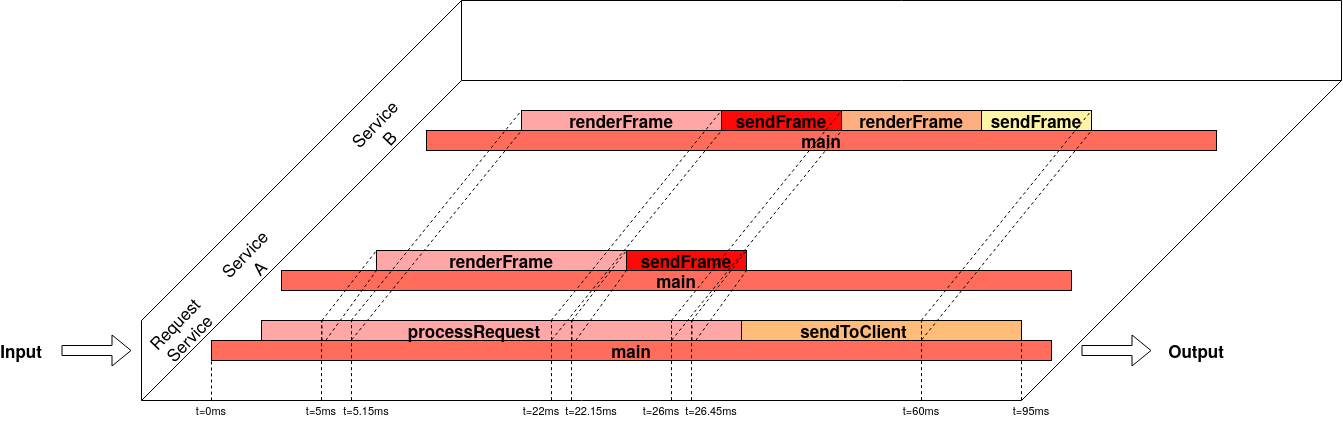
\includegraphics[scale=0.36]{img/Design/3D-Flammengraph-Konzept.png}
	\caption[Darstellungsbeispiel eines 3D-Flammengraph ]{ Darstellungsbeispiel eines 3D-Flammengraph}
	\label{fig:3D-Flammengraph-Konzept}
\end{figure}

Diese Visualisierungsform soll ein Vergleich zwischen Traces ermöglichen. Die Traces werden zusammen auf eine Zeitachse gestellt. Der Anweder kann die Traces anschließend vergleichen. Dadurch sollen nicht verwendete Frames identifizerbar sein. Auch die Ursache soll damit ermittelt werden können. Spezielle Zustände des verteilten verteilten rendering System, wie zum Beispiel dem Setzen einer neuen Kameraposition, ausgelöst durch den Client, können näher untersucht werden. Das Setzen ist eine asynchrone Funktionalität, die im rendering System dazu führt, dass eine neue Framegenerierung angestoßen wird. Dabei werden allerdings aktuell bearbeitete Frames nicht gestoppt, sondern fertiggestellt und gesendet. Diese werden nur nicht weiter verwendet. Um die zeitliche Einordnung dieser Events darstellen zu können, müssen die Traces miteinander verglichen werden. In \cref{fig:3D-Flammengraph-Vergleich} wird eine solche Situation gezeigt. Der Trace startet im Requestservice. Der Span mit dem Operationsnamen \emph{processRequest} sorgt im Render Service A für zwei Framegenerierungen. Der erste \emph{generateFrame} Span schließt zum Zeitpunkt \textbf{t1} erfolgreich ab, entsprechend wird der Frame gesendet und verwendet. Die Generierung wird mit dem zweiten generateFrame fortgesetzt. Anschließend wird der erste ProcessRequest durch eine Benutzereingabe zum Zeitpunkt \textbf{t2} unterbrochen. Der zweite Trace beginnt. Der Requestservice veranlasst die Generierung des Frames mit den neuen Benutzerdaten im Render Service B zum Zeitpunkt \textbf{t3}. Der Render Service A stellt seinen Frame zum Zeitpunkt \textbf{t4} fertig. Da der Frame auf Benutzereingaben beruht, die zu diesem Zeitpunkt veraltet sind, wird der Frame nicht weiter verwendet. Trace 1 schließt ab. Währenddessen wird Trace 2 fortgesetzt.

\begin{figure}[!ht]
	\centering
	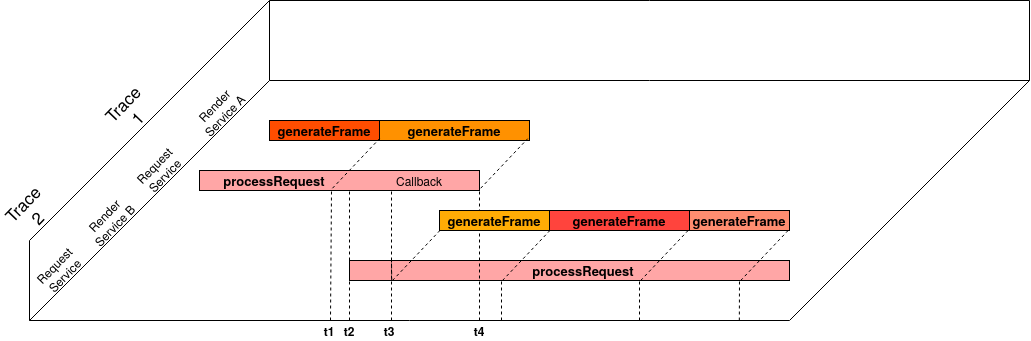
\includegraphics[scale=0.4]{img/Design/3D-Flammengraph-Vergleich.png}
	\caption[Darstellungsbeispiel eines Tracevergleich mit einem 3D Flammengraph]{ Tracevergleich mit einem 3D Flammengraph}
	\label{fig:3D-Flammengraph-Vergleich}
\end{figure}

\section{Trakorentwicklungsumgebung}
\label{section:Trakorentwicklungsumgebung}
In diesem Kapitel wird die Traktorentwicklungsumgebung spezifiziert. Die Umgebung soll die verschiedenen Anwendungsfälle der Traktorbibliothek abdecken. Eine Entwicklungsumgebung ist dahin gehend sinnvoll, dass der Anwendungsfall des verteilten rendering Systems komplexe abhängigkeiten aufweist, bei der eine effiziente Entwicklung, z.B. durch die Platformabhängigen Plugins oder der Unityumgebung, beeinträchtigt wird.

Die Traktorentwicklungsumgebung soll folgende Eigenschaften aufweisen:

\begin{itemize}
	\item \textbf{TE}.1 Die Entwicklungsumgebung soll aus mehreren Webservern bestehen
	\item  \textbf{TE}.2 Die Infrastruktur soll auf genau einem Host-System ein verteiltes System abbilden.
	\item  \textbf{TE}.3 Die Webserver-Komponenten der Entwicklungsumgebung soll mit der Traktor-API instrumentalisiert sein.
	\item  \textbf{TE}.4 Das Ansprechen der Entwicklungsumgebung soll durch einen Kommandozeilen HTTP Client ansprechbar und bedienbar sein.
\end{itemize}

Diese Spezifikation ermöglicht das Testen von Funktionalitäten der Traktor Tracingbibliothek. Dabei sollen die (\lowroman{1}) Eventgenerierungfunktionalitäten ausgeführt werden. Ausserdem soll durch durch die Instrumentalisierung von zwei miteinander kommunizierenden Komponenten (\lowroman{2}) die Kontextpropagierung durchgeführt werden. Das umfasst sowohl die lokale Kontextverwaltung, als auch die Kontextpropagierung über Prozessgrenzen hinaus. Zudem sollen die leichtgewichtigen Services, also den Reporter und die Registry, getestet werden. Dabei ist die (\lowroman{3}) Implementierung des Websocketprotokolls innerhalb der Registry, als auch der (\lowroman{4}) Websocketclient des Tracers zu untersuchen. Mit dieser Spezifikation wird ein Untersuchungssystem beschrieben, mit der teilweise die Designziele überprüft werden können. 
% ----------------------------------------------------------------------------
